\documentclass[xcolor=pdftex,hyperref={pdfpagelabels=false},table,10pt]{beamer}

\usepackage[spanish]{babel}
\usepackage[utf8]{inputenc}
\usepackage{listings}

\lstset{
   backgroundcolor=\color{lbcolor},
   tabsize=4,
   rulecolor=,
   language=C++,
       basicstyle=\scriptsize,
       upquote=true,
       columns=fixed,
       showstringspaces=false,
       extendedchars=true,
       breaklines=true,
       frame=single,
       showtabs=false,
       showspaces=false,
       showstringspaces=false,
       identifierstyle=\tt,
       keywordstyle=\color[rgb]{0.1,0.1,0.6}\bfseries,
       commentstyle=\color[rgb]{0.133,0.545,0.133},
       stringstyle=\color[rgb]{0.627,0.126,0.941},
}

\definecolor{fudepan}{HTML}{006c63}
\definecolor{verde}{RGB}{0, 127, 63}
\definecolor{gris}{RGB}{86, 86, 86}
\definecolor{listinggray}{gray}{0.9}
\definecolor{lbcolor}{rgb}{0.95,0.95,0.95}
\definecolor{azul}{RGB}{0, 110, 143}

\hypersetup{colorlinks,linkcolor=,urlcolor=verde}{}

\usetheme{Warsaw}

\usecolortheme[named=azul]{structure}

\usefonttheme{structurebold}
\useinnertheme{rounded}
\setbeamercovered{transparent}

\defbeamertemplate*{footline}{shadow theme}
{%
  \leavevmode%
  \hbox{\begin{beamercolorbox}[wd=.3\paperwidth,ht=2.5ex,dp=1.125ex,leftskip=.3cm plus1fil,rightskip=.3cm]{author in head/foot}%
    \usebeamerfont{author in head/foot}\insertframenumber\,/\,\inserttotalframenumber\hfill\insertshortauthor
  \end{beamercolorbox}%
  \begin{beamercolorbox}[wd=.7\paperwidth,ht=2.5ex,dp=1.125ex,leftskip=.3cm,rightskip=.3cm plus1fil]{title in head/foot}%
    \usebeamerfont{title in head/foot}\tesistitle
  \end{beamercolorbox}}%
  \vskip0pt%
}

\title{FuD-BOINC}
\subtitle{\tesistitle}
\author{Lucas Besso - Raúl Striglio}
\institute[UNRC]{
    \begin{minipage}{0.45\textwidth}
        \begin{center}
            %Escudo UNRC
            
\includegraphics[scale=0.23]{images/escudo.jpg}\\
            \begin{scriptsize}
                \textsc{Universidad Nacional de Río Cuarto} \\
            \end{scriptsize}
            \vfill
            \begin{tiny}
                \textsc{Fac. de Cs. Exactas, Fco-Qcas y Naturales} \\
                \textsc{Departamento de Computación} \\[1cm]
            \end{tiny}
        \end{center}
    \end{minipage}
    \begin{minipage}{0.45\textwidth}
        \begin{center}
            %Escudo FuDePAN
            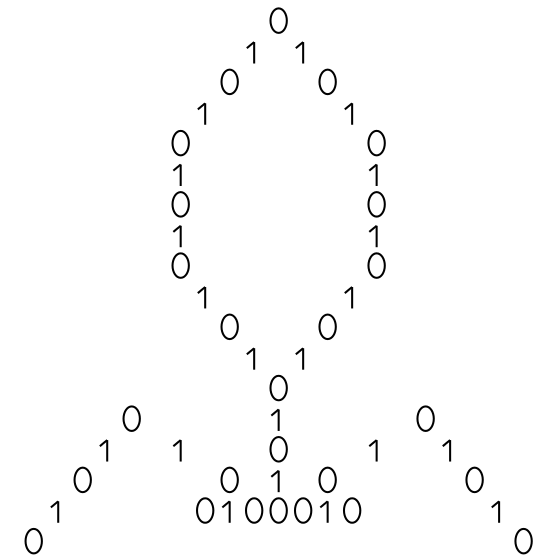
\includegraphics[scale=0.1]{images/logo-fudepan.png}\\
            \vfill
            \begin{scriptsize}
                \textsc{FuDePAN} \\
            \end{scriptsize}
            \begin{tiny}
                \textsc{Fundación para el Desarrollo de la Programación en Ácidos Nucleicos} \\[0.5cm]
            \end{tiny}
        \end{center}
    \end{minipage}
}
\date{28 de Diciembre de 2011}

\newcommand{\fudepan}{\textbf{FuDePAN}}
\newcommand{\fud}{\textbf{FuD}}
\newcommand{\tesistitle}{Implementación de una capa de distribución del framework FuD utilizando como middleware a BOINC}

\begin{document}

\begin{frame}
    \titlepage
\end{frame}


\begin{frame}
    \frametitle{Temario}
   \scriptsize{ \tableofcontents }
\end{frame}

\chapter{Introducción}
\label{chapter:introduccion}

Hoy en día son cada vez más las entidades sin fines de lucro que realizan determinadas investigaciones científicas con el objetivo de aportar un gran avance o descubrimiento en distintas áreas tales como la medicina, Astronomía, Física, Química, etc. Tal es el caso de la organización sin fines de lucro FuDePAN\footnote{\url{http://www.fudepan.org.ar/}} (Fundación para el Desarrollo de la Programación en Ácidos Nucleicos) la cual se dedica a la investigación y desarrollo en bioinformática aplicada a problemas biológicos asociados a la salud humana. En esta fundación utilizan el cálculo computacional para hacer simulaciones sobre cómo determinados virus y enfermedades, tales como el HIV o el virus Junín, actúan en el cuerpo humano con el fin de mejorar los tratamientos y las vacunas contra los mismos.

Los problemas que generalmente son enfrentados en FuDePAN son de alta complejidad por lo que se requiere un gran poder computacional para poder resolverlos en el menor lapso de tiempo posible. Es por eso que se desarrolló el framework FuD\footnote{\url{http://code.google.com/p/fud/}} (Ubiquitous Distribution Platform) para la distribución automática de trabajos en nodos de procesamiento, el cual permite obtener soluciones paralelizadas a partir de proyectos secuenciales realizando una simple reimplementación. Mediante el uso de este framework se lograron obtener resultados confiables en lapsos de tiempo relativamente cortos.

En sus orígenes, la capa de distribución de FuD sólo fue implementada con la librería de E/S asincrónica de Boost\footnote{\url{http://www.boost.org/}} (o Boost::asio) con el objetivo de poder realizar computación de alto rendimiento. Sin embargo, para poder aprovechar al máximo dicha implementación se requería de un tipo de súper-computadora la cual era muy costosa. Es por ello que surge la motivación de poder implementar una nueva capa de distribución de FuD con el middleware para la computación voluntaria BOINC, con el fin de poder obtener un mayor poder de procesamiento a un costo significativamente menor gracias a personas voluntarias que donan los recursos ocioso de sus computadoras personales para realizar computación científica.

El objetivo de este proyecto fue poder acoplar el funcionamiento de la capa de distribución del framework FuD con la plataforma BOINC para permitirle a los usuarios de FuD contar con la posibilidad de ejecutar sus aplicaciones sobre un proyecto para la computación voluntaria. De esta manera, FuD cuenta con una variante para realizar computación de alto rendimiento y otra para la computación voluntaria.

Este documento ofrece una visión general de las tareas de investigación realizadas, del diseño, de algunos detalles de implementación y de algunas pruebas realizadas. Se muestran distintos ejemplos que facilitaron la comprensión de las tareas mencionadas anteriormente, como así también los resultados de ejecutar ciertas aplicaciones compiladas con esta nueva implementación de FuD.

El informe se divide en 5 partes. La parte  “Preliminar” incluye: una introducción a este trabajo (\ref{chapter:introduccion}), un capítulo con el marco teórico (\ref{chapter:marco:teorico}) para facilitar la lectura de este documento y otro capítulo con la metodología de trabajo (\ref{chapter:metodologia}) utilizada para desarrollar el proyecto.
	 	 	
La parte “Capa de distribución FuD-BOINC” contiene todo lo relacionado sobre este proyecto \ref{chapter:sobre:fud:boinc}. Se enuncia el problema y el enfoque de solución abordado para luego ofrecerle al lector detalles de diseño (\ref{chapter:diseno}) e implementación (\ref{chapter:implementacion}), como así también de las pruebas realizadas (\ref{chapter:pruebas}) y los resultados obtenidos (\ref{chapter:resultados}).

La parte “Conclusión” presenta la conclusión (\ref{chapter:conclusion}) que se pudo obtener luego de realizar este proyecto y los trabajos a futuro (\ref{chapter:future:work}) relacionados al mismo.

La parte “Bibliografía”, como bien indica su nombre, muestra la bibliografía (\ref{biblio}) utilizada, y finalmente, la parte “Apéndices” muestra un reporte completo de métricas de código (\ref{chapter:FuD-BOINC:metrics_report}).
\section{FuD-BOINC}

\begin{subsection}{¿Qué es FuD-BOINC?}

	\begin{frame}\frametitle{¿Qué es FuD-BOINC?}	
		\begin{itemize}
		\item Una nueva implementación de la capa L1 de \fud .
		\item Permite que aplicaciones desarrolladas con \fud \ puedan correr sobre proyectos BOINC.
		\item Permite abstraer al desarrollador de aplicaciones \fud \ de la API de BOINC.
		\end{itemize}
		
		\begin{center}
			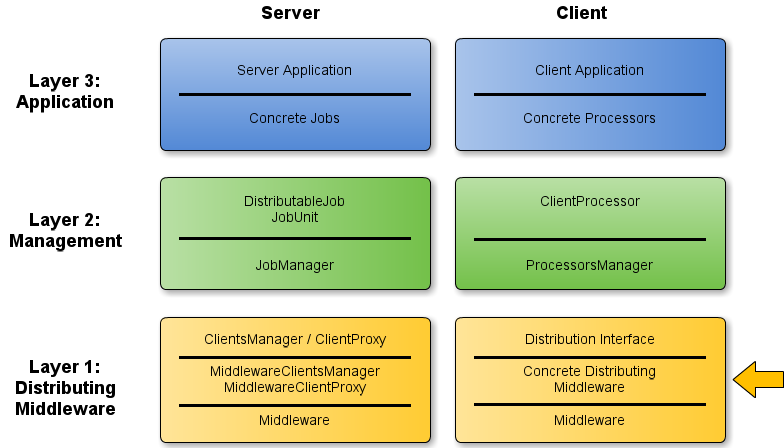
\includegraphics[scale=0.27]{images/AbstractLayers-FuD-L1.png}
		\end{center}
	\end{frame}
	
\end{subsection}
				

\begin{subsection}{Diseño}

	\begin{frame}\frametitle{Capa de distribución: lado servidor}
		\begin{center}
			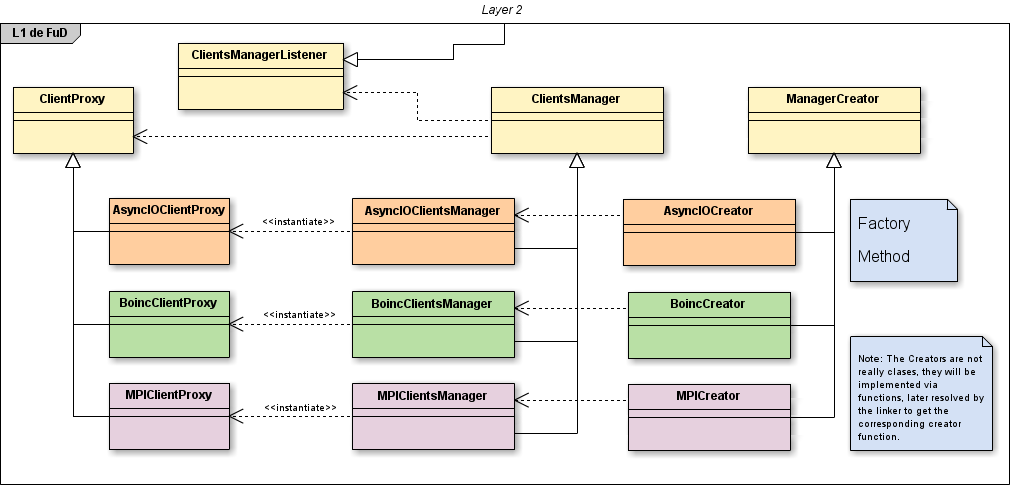
\includegraphics[scale=0.31]{images/diseno-servidor-fud.png}
		\end{center}
	\end{frame}
	
	\begin{frame}\frametitle{Lado servidor: \texttt{BoincClientsManager}}
  		\begin{figure}[h]
    		\begin{minipage}{3.3cm}
      			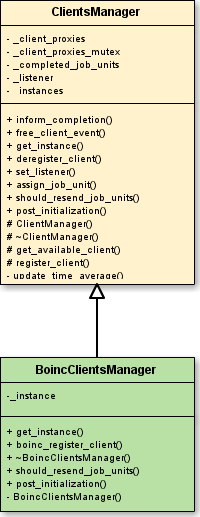
\includegraphics[scale=0.35]{images/BoincClientsManager.png}
    		\end{minipage}
    		\begin{minipage}{0.67 \textwidth}
				\begin{block}{\texttt{BoincClientsManager}}
      				Hereda de la clase \texttt{ClientsManager} de \fud .
      			\end{block}
      			\vspace{7mm}
      			\begin{block}{Responsabilidades}
      				\begin{itemize}
						\item Realizar el registro de un único cliente.
						\item Comunicar al manejador de trabajos la disponibilidad del cliente conectado.
					\end{itemize}
      			\end{block}	
      		\end{minipage}
    	\end{figure}
	\end{frame}
	
	\begin{frame}\frametitle{Lado servidor: \texttt{BoincClientProxy}}
  		\begin{figure}[h] 		
    		\begin{minipage}{2.7cm}
      			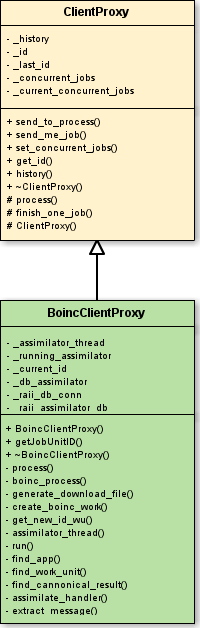
\includegraphics[scale=0.3]{images/BoincClientProxy.png}
    		\end{minipage}
    		\begin{minipage}{0.7 \textwidth}
      			\begin{block}{\texttt{BoincClientProxy}}
      				Hereda de la clase \texttt{ClientProxy} de \fud \ y representa un cliente conectado con la 
      				particularidad que siempre está disponible.
      			\end{block}
				\vspace{3mm}
      			\begin{block}{Responsabilidades}
      				\begin{itemize}
						\item Mantener una conexión directa con la base de datos del proyecto BOINC.
						\item Generar un trabajo de BOINC a partir de una \texttt{JobUnit}.
						\item Obtener los resultados enviados por los clientes e informarlos a L2.
					\end{itemize}
      			\end{block}	
      		\end{minipage}
    	\end{figure}
	\end{frame}

	\begin{frame}\frametitle{Capa de distribución: lado cliente}
		\begin{center}
			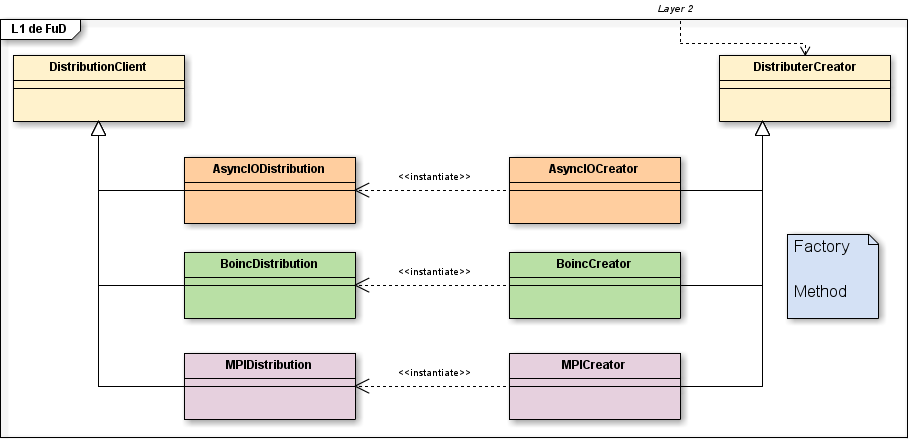
\includegraphics[scale=0.35]{images/diseno-cliente-fud.png}
		\end{center}
	\end{frame}

	\begin{frame}\frametitle{Lado cliente: \texttt{BoincDistribution}}
  		\begin{figure} 		
    		\begin{minipage}{0.2\linewidth}
      			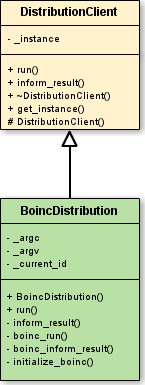
\includegraphics[scale=0.5]{images/BoincDistribution.png}
    		\end{minipage}
    		\hfill
    		\begin{minipage}{0.7\linewidth}
      			\begin{block}{\texttt{BoincDistribution}}
      				Hereda de la clase DistributionClient de \fud \ y provee la funcionalidad necesaria para que la aplicación pueda correr 					satisfactoriamente sobre el cliente BOINC.
      			\end{block}
				\vspace{2mm}
      			\begin{block}{Responsabilidades}
      				\begin{itemize}
      					\item Extraer la \texttt{JobUnit} del archivo de entrada brindado por el \textbf{cliente de BOINC}.
						\item Envíar la \texttt{JobUnit} a la capa L2 para su procesamiento.
						\item Escribir el resultado de la tarea en un archivo de salida para que el \textbf{cliente de BOINC} 
						lo informe al servidor.
					\end{itemize}
      			\end{block}	
      		\end{minipage}
    	\end{figure}
	\end{frame}

\end{subsection}


\begin{subsection}{Implementación}

	\begin{frame}[fragile]\frametitle{API de BOINC}
		\begin{block}{Servidor}
			Del lado servidor de FuD-BOINC se debió utilizar la API de BOINC para realizar las siguientes tareas:
			\vspace{1mm}
			\begin{itemize}
				\item Leer el archivo de configuración del proyecto BOINC:
					\begin{lstlisting}
						config.parse_file()
					\end{lstlisting}
				\item Establecer una conexión con la base de datos:
					\begin{lstlisting}
						boinc_db.open(config.db_name, config.db_host, config.db_user, config.db_passwd);
					\end{lstlisting}
			\end{itemize}
		\end{block}
	\end{frame}

	\begin{frame}[fragile]\frametitle{API de BOINC}
		\begin{block}{Cliente}
			Del lado cliente de FuD-BOINC se debió utilizar la API de BOINC para realizar las siguientes tareas:
			\vspace{2mm}
			\begin{itemize}
				\item Inicializar los diagnósticos de BOINC:
					\begin{lstlisting}
						int boinc_init_diagnostics(int flags);
					\end{lstlisting}
				\item Inicializar la aplicación cliente de BOINC para que sea propiamente ejecutada por el cliente de BOINC:
					\begin{lstlisting}
						boinc_init();
          			\end{lstlisting}
				\item Finalizar la aplicación cliente de BOINC:
         			\begin{lstlisting}
						int boinc_finish(int status);
          			\end{lstlisting}
    		\end{itemize}
  		\end{block}
	\end{frame}

	\begin{frame}\frametitle{Servidor: envío de trabajos}
		\begin{block}{}
			\fud \ provee el método \texttt{process()} mediante el cual se envían \texttt{JobUnits} a clientes.
		\end{block}
		\vspace{5mm}
		\pause
		En FuD-BOINC, el método \texttt{process()} se encarga de traducir una \texttt{JobUnit} a un trabajo de BOINC
		mediante los siguientes pasos:
		\vspace{5mm}
		\begin{enumerate}
		\addtolength{\itemsep}{2mm}
			\item Serializar la \texttt{JobUnit} de \fud \ dentro de un archivo binario.
			\item Leer la plantilla utilizada por BOINC en donde se especifican las características de la \textbf{workunit} a crear.
			\item Invocar al método \texttt{create\_boinc\_work()}.
		\end{enumerate}
	\end{frame}

	\begin{frame}[fragile]\frametitle{Servidor: crear trabajo de BOINC}
		\begin{block}{create\_boinc\_work()}
			El método \texttt{create\_boinc\_work()} es el encargado de crear un nuevo trabajo de BOINC.
		\end{block}
		Las tareas llevadas a cabo por éste método se pueden simplificar en los siguientes pasos:
		\begin{enumerate}
			\item Crear el nombre que identifica la \textbf{workunit}.
			\item Asociar la nueva tarea a la aplicación en ejecución.
			\item Crear el trabajo invocando al método \texttt{create\_work()} de BOINC.
		\end{enumerate}
		\vspace{2mm}
		\begin{lstlisting}[frame=single]   
			create_work( wu, wu_template,
			             RE_TEMPLATE.c_str(),
			             config.project_path(RE_TEMPLATE.c_str()),
			             input_files, NRO_INFILES, config );
		\end{lstlisting}
	\end{frame}

	\begin{frame}\frametitle{Servidor: obtener resultados de clientes}
		\begin{block}{}
			\fud \ provee el método \texttt{inform\_completion()} para informar los resultados de las \texttt{JobUnit} 
			recibidos desde los clientes a las capas superiores.
		\end{block}
		\vspace{2mm}
		\pause
		\begin{block}{}
			Para recibir y manejar los resultados enviados por los clientes de BOINC, se debió integrar 
			el comportamiento del demonio \textit{\textbf{assimilator}} como parte del comportamiento de FuD-BOINC.
		\end{block}
		\vspace{2mm}
		\pause
		\begin{block}{¿Cómo?}
			Se implementó un nuevo hilo de ejecución dentro del servidor FuD-BOINC para que se encargue de chequear 
			la existencia de nuevos resultados no asimilados.
		\end{block}
	\end{frame}

	\begin{frame}[fragile]\frametitle{Servidor: asimilador de tareas}
		\begin{block}{}
			El thread assimilator cumple con las siguientes funciones:
			\vspace{2mm}
			\begin{itemize}
				\item Buscar en la base de datos workunits no asimiladas
				\item Verificar si se encontró resultado canónico para dichas workunits
				\item Invocar al método \texttt{assimilate\_handler()}, una vez confirmada la existencia de un resultado canónico
			\end{itemize}
		\end{block}
		\pause
		\vspace{4mm}
		\begin{block}{assimilate\_handler()}
			Extrae el resultado de la workunit del archivo de salida enviado por el cliente BOINC para luego informarlo 
			mediante el método \texttt{inform\_completion()} de FuD.
		\end{block}
	\end{frame}

	\begin{frame}[fragile]\frametitle{Servidor: asimilador de tareas}
		\textbf{Ciclo del \texttt{assimilator\_thread()}:}
		\begin{lstlisting}
	app = find_app(NAME_APP, _db_assimilator);
	while(_running_assimilator)
	{
	    if (find_work_unit(app, wu) == true)
	    {
	        if ( find_cannonical_result(wu,canonical_result) == true )
	        {
	            assimilate_handler(wu,canonical_result);
	            update_wu_state(wu, WuDone);
	        }
	     }
	     sleep(SLEEP_INTERVAL);
	}
		\end{lstlisting}
		\textbf{Tareas más relevantes del método \texttt{assimilate\_handler()}:}
		\begin{lstlisting}
			std::string* msg = extract_message(output_file);
			ClientsManager::get_instance()->inform_completion(getJobUnitID(), msg);
		\end{lstlisting}
	\end{frame}

	\begin{frame}\frametitle{Cliente: computación de una tarea}
		\begin{block}{}
			\fud \ provee el método \texttt{run()} el cual debe ser implementado con las tareas específicas que debe 
			realizar el cliente para llevar a cabo el cómputo de las JobUnits.
		\end{block}
		\pause
		\vspace{4mm}
		En FuD-BOINC, el método \texttt{run()} se remite a obtener la \texttt{JobUnit} de \fud \ a partir del trabajo 
		de BOINC mediante los siguientes pasos:
		\vspace{4mm}
		\begin{enumerate}\addtolength{\itemsep}{2mm}
		    \item Leer el archivo binario que contiene encapsulada la JobUnit de FuD
		    \item Extraer el mensaje correspondiente a la JobUnit de FuD
		    \item Invocar al método \texttt{deliver\_message()} quien enviará el contenido a las capas superiores para su computación.
		\end{enumerate}
	\end{frame}

	\begin{frame}\frametitle{Cliente: informar resultado}
		\begin{block}{}
			\fud \ provee el método \texttt{inform\_result()} cuya función es enviar el resultado de la computación al servidor.
		\end{block}
		\pause
		\vspace{6mm}
		En FuD-BOINC se remite a invocar al método \texttt{boinc\_inform\_result()} el cual se encarga de las siguientes tareas:
		\vspace{4mm}
		\begin{enumerate}\addtolength{\itemsep}{3mm}
			\item Obtener el resultado de la computación
			\item Escribir dicho resultado en un archivo de salida asociado al trabajo de BOINC
		\end{enumerate}
	\end{frame}

	\begin{frame}[fragile]\frametitle{Cliente: informar resultado}
		Parte del código de \texttt{boinc\_inform\_result()}:
		\vspace{4mm}
			\begin{lstlisting}
		std::string body = ProcessorsManager::get_instance()->get_return_message();
	
		OutputMessage bos;
		bos << _current_id << body;
	
		// File to upload to server.
		std::ofstream out;
	
		//enable the exceptions
		out.exceptions ( std::ofstream::failbit | std::ofstream::badbit );
		out.open(file_name.c_str(), std::ios::binary);
	
		// Get the message with result of computation to send back to server
		out << bos.str();
			\end{lstlisting}
	\end{frame}

	\begin{frame}\frametitle{Cliente: compilación en Windows}
		\begin{block}{}
			Fue necesario compilar el cliente de FuD-BOINC para sistemas operativos Windows ya que actualmente son los más utilizados.
		\end{block}
		\begin{block}{}
			Pasos para la compilación:
			\vspace{2mm}
			\begin{enumerate}\addtolength{\itemsep}{1mm}
				\item Compilar las librerías BOINC.
				\item Generar y configurar un proyecto solución de \textit{Visual Studio} para la compilación de FuD-BOINC.
				\item Resolver dependencias con las librerías: boost, pthread, mili y MySQL
				\item Modificar el tipo de \texttt{include} realizado en algunos archivos del cliente \fud.
				\item Compilar el cliente de \fud.
			\end{enumerate}		
		\end{block}
	\end{frame}

\end{subsection}


\begin{subsection}{Interacción entre FuD y BOINC}

	\begin{frame}\frametitle{Servidor: envío de una \texttt{JobUnit}}
		\begin{center}
			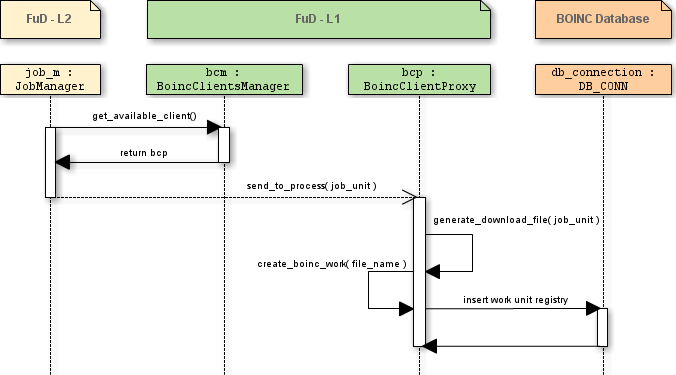
\includegraphics[scale=0.45]{images/interaccion-fud-boinc-server_side.png}
		\end{center}
	\end{frame}
	
	\begin{frame}\frametitle{Cliente: computación de una \texttt{JobUnit}}
		\begin{center}
			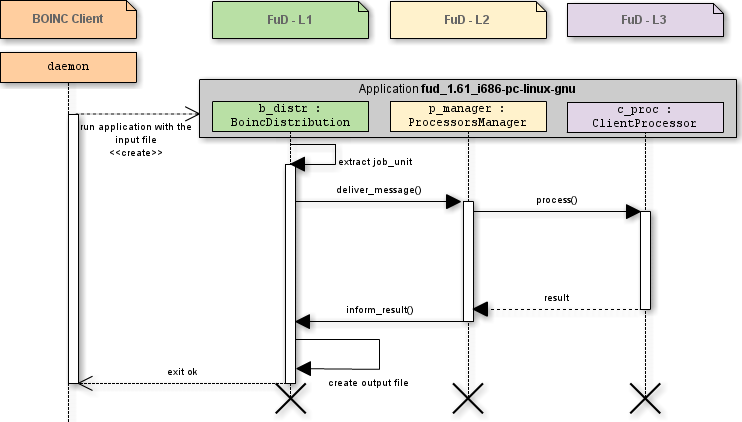
\includegraphics[scale=0.4]{images/interaccion-fud-boinc-client_side.png}
		\end{center}
	\end{frame}

\end{subsection}


\section{Rediseño de FuD}


\begin{frame}\frametitle{Rediseño de FuD}	
	\begin{block}{}
		Durante el desarrollo de este proyecto se debieron efectuar diversos cambios en el diseño e implementación 
		original de FuD para poder integrar esta nueva capa de distribución.
	\end{block}
	\vspace{4mm}
	\begin{itemize}\addtolength{\itemsep}{4mm}
		\item Redeclaración del método \texttt{create\_distribution\_client()}
		\item \texttt{JobManager} post initialization
		\item Reenvío de \texttt{JobUnits} configurable
		\item Múltiples \texttt{JobUnits} a clientes
	\end{itemize}
\end{frame}


\begin{subsection}{Redeclaración del método \texttt{create\_distribution\_client()}}

	\begin{frame}[fragile]\frametitle{Redeclaración del método \texttt{create\_distribution\_client()}}	
		\begin{block}{}
			Método provisto por \fud \ para la creación de un cliente de distribución.
		\end{block}
		\vspace{4mm}
		Prototipo original:
		\begin{lstlisting}
		DistributionClient* create_distribution_client(
		        std::string address = "127.0.0.1", Port port = 31337);
		\end{lstlisting}
		\vspace{4mm}		
		Prototipo actual:
		\begin{lstlisting}
		DistributionClient* create_distribution_client(
		        int argc, char** argv);
   		\end{lstlisting}
	\end{frame}

\end{subsection}


\begin{subsection}{\texttt{JobManager} post initialization}

	\begin{frame}[fragile]\frametitle{\texttt{JobManager} post initialization}
  		\begin{figure}[h] 		
    		\begin{minipage}{0.26 \textwidth}
      			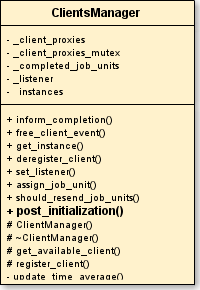
\includegraphics[scale=0.5]{images/ClientsManager-post-init.png}
    		\end{minipage}
    		\hfill
    		\begin{minipage}{0.64 \textwidth}
      			\begin{block}{}
      				\begin{itemize}\addtolength{\itemsep}{6mm}
						\item Se agregó un nuevo método en la clase \texttt{ClientsManager} de \fud.
						\item Por defecto, su implementación es vacía.
						\item El método sólo es invocado al final del constructor de \texttt{JobManager}:
						\begin{lstlisting}
							_clients_manager->post_initialization()
						\end{lstlisting}
					\end{itemize}
      			\end{block}
      		\end{minipage}
      	\end{figure}
	\end{frame}
	
	\begin{frame}[fragile]\frametitle{Redefinición de \texttt{post\_initialization()}}
		\begin{block}{Declaración y definición en \texttt{ClientsManager}}
			\begin{lstlisting}
				virtual void post_initialization() {};
			\end{lstlisting}
		\end{block}
		
		\begin{block}{Redefinición en \texttt{BoincClientsManager}}
			\begin{lstlisting}
				void BoincClientsManager::post_initialization()
				{    boinc_register_client();    }
			\end{lstlisting}
			\begin{lstlisting}
				void BoincClientsManager::boinc_register_client()
				{
				    // Init the client_proxy.
				    boinc_log_debug(std::string("Registering BOINC with FuD."));
				    BoincClientProxy * client = new BoincClientProxy();
				    client->set_concurrent_jobs(UNLIMITED_JOBS);
				    // Register the unique client proxy.
				    register_client(client);
				}
			\end{lstlisting}
		\end{block}
	\end{frame}

\end{subsection}


\begin{subsection}{Reenvío de \texttt{JobUnits} configurable}

	\begin{frame}[fragile]\frametitle{Reenvío de \texttt{JobUnits} configurable}
  		\begin{figure}[h] 		
    		\begin{minipage}{0.26 \textwidth}
      			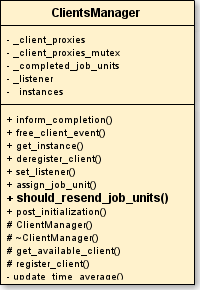
\includegraphics[scale=0.5]{images/ClientsManager-resend-jobunit.png}
    		\end{minipage}
    		\hfill
    		\begin{minipage}{0.64 \textwidth}
      			\begin{block}{}
      				\begin{itemize}\addtolength{\itemsep}{4mm}
						\item Se agregó un nuevo método en la clase \texttt{ClientsManager} de \fud.
							\begin{lstlisting}[basicstyle=\tiny]
								virtual bool should_resend_job_units() = 0;
							\end{lstlisting}
						\item Definición del método en \texttt{BoincClientsManager}:
							\begin{lstlisting}[basicstyle=\tiny]
								bool BoincClientsManager::should_resend_job_units()
								{
								    return false;
								}
							\end{lstlisting}
					\end{itemize}
      			\end{block}
      		\end{minipage}
      	\end{figure}
	\end{frame}
	
	\begin{frame}[fragile]\frametitle{Reimplementación de \texttt{handle\_free\_client\_event()}}
  		\begin{lstlisting}[basicstyle=\tiny, numbers=left, firstnumber=170]
	if (_jobQueue.empty())
	{
	    if (_clients_manager->should_resend_job_units()) 
	    {
	        if (! _pendingList.empty())
	        {
	            if (_clients_manager->assign_job_unit(*_pendingList.front()))
	            {
	                //send this one to the back, act as Round Robin
	                _pendingList.push_back(_pendingList.front());
	                _pendingList.pop_front();
	            }
	            else
	                syslog(LOG_NOTICE, "Error sending JobUnit %u from Pending List to a client.", _pendingList.front()->get_id());
	        }
	    }
	}
	else
	{
	    if (_clients_manager->assign_job_unit(*_jobQueue.front()))
	    {
	        syslog(LOG_NOTICE, "Sending JobUnit %u to pending list.", (_jobQueue.front()->get_id()));
	        _pendingList.push_back(_jobQueue.front());
	        _jobQueue.pop_front();
	    }
	    else
	        syslog(LOG_NOTICE, "Error sending JobUnit %u from Job Queue to a client.", _jobQueue.front()->get_id());
	}	
  		\end{lstlisting}
	\end{frame}
	
\end{subsection}


\begin{subsection}{Múltiples \texttt{JobUnits} a clientes}

	\begin{frame}\frametitle{Múltiples \texttt{JobUnits} a clientes}
		\begin{block}{Problema}
			Los clientes sólo pueden procesar a lo sumo de a una JobUnit por vez.
		\end{block}
		\pause
		\begin{block}{Solución}
			La idea general consiste en:
			\begin{enumerate}\addtolength{\itemsep}{2mm}
				\item Permitir configurar la cantidad máxima de tareas en simultáneo que un cliente puede ejecutar. \pause
				\item Llevar un registro de la cantidad de tareas que un cliente se encuentra computando en un determinado momento.\pause
				\item Determinar la disponibilidad de un cliente.\pause
				\item Si el cliente se encuentra disponible, generar un nuevo evento de cliente libre.
			\end{enumerate}
		\end{block}
	\end{frame}

	\begin{frame}\frametitle{ClientProxy}
		\begin{figure}
      		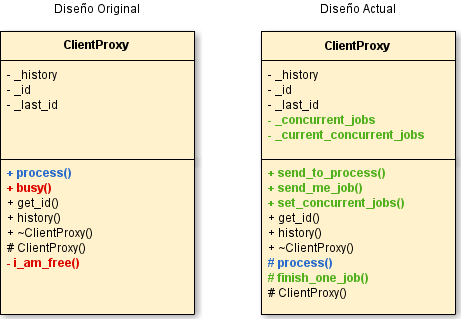
\includegraphics[scale=0.5]{images/ClientProxy-orig-vs-actual.png}
      	\end{figure}
	\end{frame}

	\begin{frame}\frametitle{ClientsManager}
		\begin{figure}
      		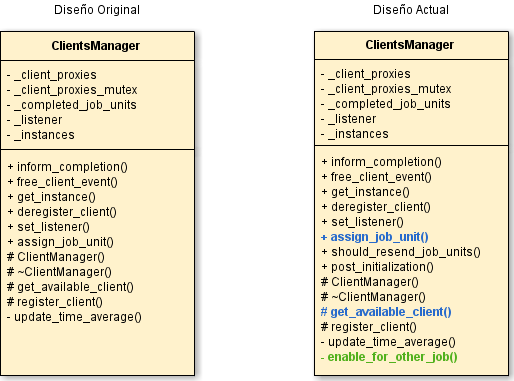
\includegraphics[scale=0.5]{images/ClientsManager-orig-vs-actual.png}
      	\end{figure}
	\end{frame}

	\begin{frame}\frametitle{Diagrama de secuencia: multiple jobs}
		\begin{figure}
      		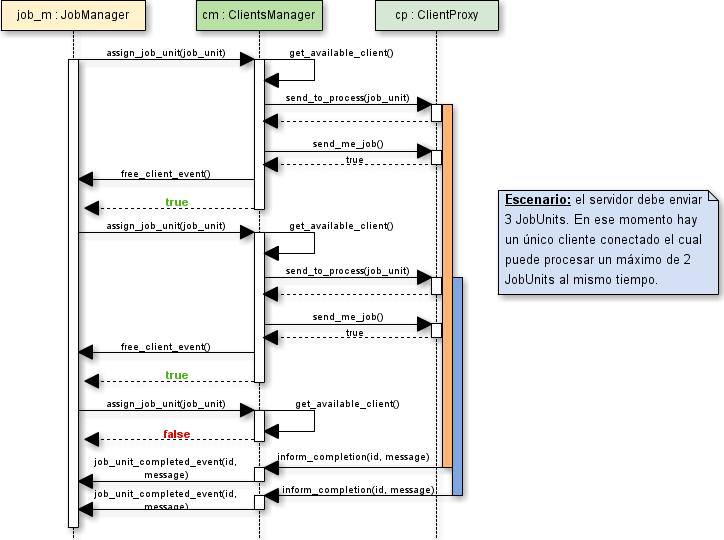
\includegraphics[scale=0.38]{images/diagr-sec-rediseno-mult-jobs.png}
      	\end{figure}
	\end{frame}



\end{subsection}

\section{Aplicación de prueba}

\begin{subsection}{Parallel-Clusterer}
\begin{frame}\frametitle{Parallel-Clusterer}

\begin{block}{Parallel-clusterer}
Es una aplicación utilizada por la organización FuDePAN. Fue desarrollada utilizando el framework FuD y realiza la siguiente tarea:
\end{block}

\pause
\vspace{2mm}
\begin{block}{Tarea:}
Dado un conjunto de diferentes cadenas principales o esqueletos de una proteína (cada uno representado por un vector de átomos), agrupa estos elementos bajo similitudes geométricas de las posiciones de sus átomos.

El resultado final es un conjunto de agrupaciones o clusters donde cada uno tiene esqueletos de proteínas cuya estructura geométrica es muy similar.
\end{block}
\end{frame}

\begin{frame}\frametitle{Parallel-clusterer}

\textbf{Estructura de un esqueleto de proteína:}
\begin{center}
	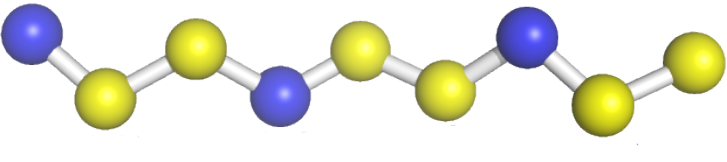
\includegraphics[scale=0.2]{images/backbone.png}
\end{center}

\textbf{Clusters resultantes:}

	\begin{minipage}{3cm}
		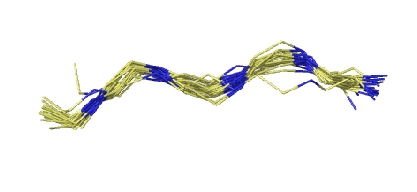
\includegraphics[scale=0.35]{images/grafico_cluster.jpg}
    \end{minipage}
    \    \ \hfill
	\begin{minipage}{5cm}
	    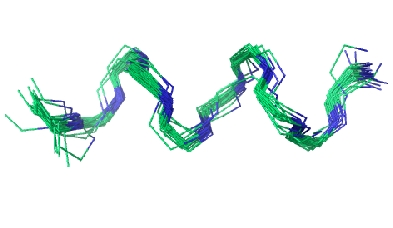
\includegraphics[scale=0.35]{images/grafico_cluster1.jpg}
	\end{minipage}
\end{frame}
\end{subsection}

\begin{subsection}{Análisis de rendimiento}
\begin{frame}\frametitle{Análisis de rendimiento}

\begin{block}{}
Es importante realizar el análisis de rendimiento de una aplicación distribuida con el propósito de estudiar los costos/beneficios que ésta posee ante la comparación con su versión secuencial.
\end{block}

\begin{block}{}
Se muestra el análisis de rendimiento de la aplicación Parallel-Clusterer compilada con FuD-BOINC en términos de las siguientes métricas:

\begin{itemize}
\item Aceleración
\item Eficiencia
\item Overhead
\item Costo
\end{itemize}

La ejecución se llevo a cabo variando de 1 a 5 clientes conectados.

\end{block}

\end{frame}

\begin{frame}\frametitle{Tiempo de ejecución}

\begin{block}{Tiempo secuencial (\textbf{$T_s$})}
Se define como el intervalo de tiempo que transcurre desde que un programa secuencial se inicia hasta que finaliza.
\end{block}

\pause
\begin{block}{Tiempo distribuido (\textbf{$T_p$})}
Se calcula desde que se inicia hasta que el último nodo finaliza su ejecución.
\end{block}

\pause
\begin{block}{}
Factores que afectaron al tiempo de ejecución de la aplicación distribuida:

\begin{itemize}
\item Tiempo de descarga de archivos de entrada y de la aplicación.
\item Tiempo de subida de los archivos resultantes.
\item Tiempo entre requerimientos al servidor.
\end{itemize}

\end{block}
\end{frame}

\begin{frame}\frametitle{Tiempo de ejecución}

\textbf{Tiempo secuencial (\textit{T$_{s}$}) vs. Tiempo paralelo (\textit{T$_{p}$})}

\vspace{2mm}
T$_{s}$ = 110.7 segundos.
\begin{center}
\begin{figure}[!ht]
    %Tabla & Grafico
    \begin{minipage}{2,0cm}
    \begin{flushleft}
    \begin{tabular*}{1,8cm}{c@{\extracolsep{\fill}}c}
        \hline
        \textbf{p} & \textbf{$T_p$} \\ \hline 
        1 & 305 \\ \hline
        2 & 249 \\ \hline
        3 & 259 \\ \hline
        4 & 245 \\ \hline
        5 & 222 \\ \hline
    \end{tabular*}
    \end{flushleft}
    \end{minipage}
    \    \ \hfill
    \begin{minipage}{8cm}
    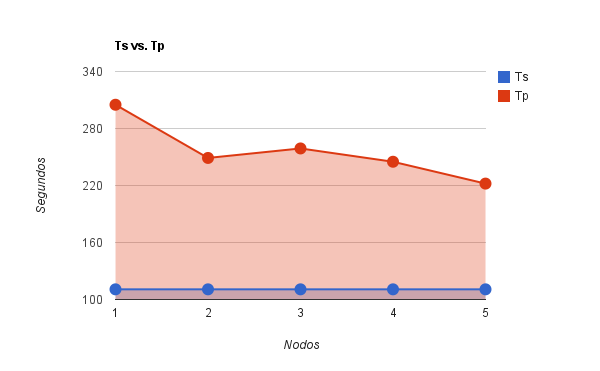
\includegraphics[scale=0.4]{images/Grafico_de_tiempos.png}\\
    \end{minipage}
\end{figure}
\end{center}
\end{frame}

\begin{frame}\frametitle{Aceleración}

\begin{block}{Definición}
Es una medida que arroja el beneficio relativo de resolver un problema en paralelo. Indica la ganancia de velocidad obtenida.
\end{block}

Se define como: \textit{S} = \textit{T$_{s}$}/\textit{T$_{p}$}

\begin{center}
\begin{figure}[!ht]
    %Tabla & Grafico
    \begin{minipage}{2,0cm}
    \begin{flushleft}
    \begin{tabular*}{1,8cm}{c@{\extracolsep{\fill}}c}
        \hline
        \textbf{p} & \textbf{$S$} \\ \hline 
        1  & 0.36 \\ \hline
        2  & 0.44 \\ \hline
        3  & 0.42 \\ \hline
        4  & 0.45 \\ \hline
        5  & 0.49 \\ \hline
    \end{tabular*}
    \end{flushleft}
    \end{minipage}
    \    \ \hfill
    \begin{minipage}{8cm}
    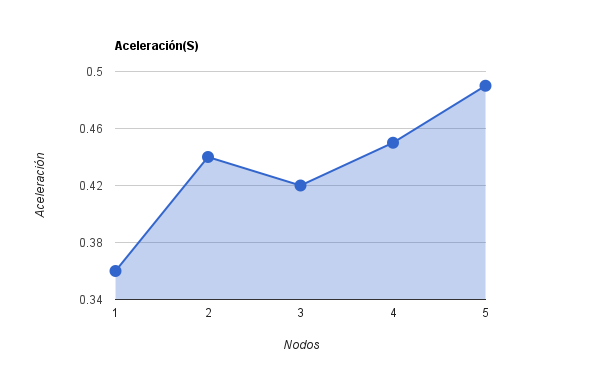
\includegraphics[scale=0.35]{images/Grafico_Aceleracion.png}\\
    \end{minipage}
\end{figure}
\end{center}

\end{frame}

\begin{frame}\frametitle{Eficiencia}

\begin{block}{Definición}
Indica el grado de utilidad de cada elemento de procesamiento.
\end{block}
Se define como: \textit{E} = \textit{S}/\textit{p}

\begin{center}
\begin{figure}[H]
    %Tabla & Grafico
    \begin{minipage}{2,0cm}
    \begin{flushright}
    \begin{tabular*}{1,8cm}{c@{\extracolsep{\fill}}c}
        \hline
        \textbf{p} & \textbf{$E$} \\ \hline 
        1  & 0.36 \\ \hline
        2  & 0,22 \\ \hline
        3  & 0,14 \\ \hline
        4  & 0,11 \\ \hline
        5  & 0,09 \\ \hline
    \end{tabular*}
    \end{flushright}
    \end{minipage}
    \    \ \hfill
    \begin{minipage}{8cm}
    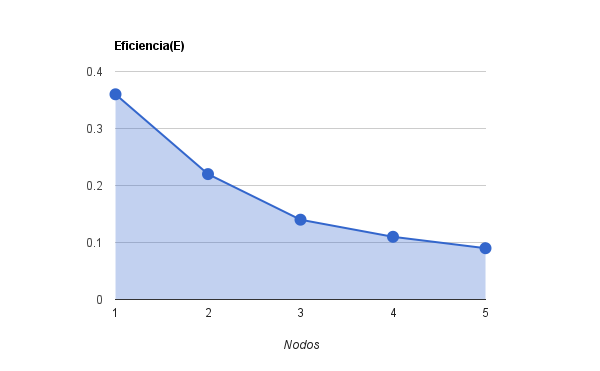
\includegraphics[scale=0.35]{images/Grafico_Eficiencia.png}\\
    \end{minipage}
\end{figure}
\end{center}

\end{frame}

\begin{frame}\frametitle{Overhead}

\begin{block}{Definición}
Indica el trabajo adicional que realiza un programa paralelo respecto a la solución secuencial equivalente.

\end{block}
Se define como: \textit{T$_{o}$} = \textit{p} $_*$ \textit{T$_{p}$} $_-$ \textit{T$_{s}$}

\begin{center}
\begin{figure}[H]
    %Tabla & Grafico
    \begin{minipage}{2,0cm}
    \begin{flushright}
    \begin{tabular*}{1,8cm}{c@{\extracolsep{\fill}}c}
        \hline
        \textbf{p} & \textbf{$T_0$} \\ \hline 
        1  & 194.3 \\ \hline
        2  & 387.3 \\ \hline
        3  & 666.3 \\ \hline
        4  & 869.3 \\ \hline
        5  & 999.3 \\ \hline
    \end{tabular*}
    \end{flushright}
    \end{minipage}
    \    \ \hfill
    \begin{minipage}{8cm}
    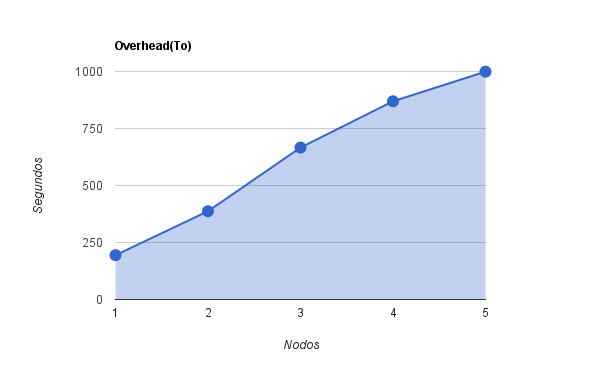
\includegraphics[scale=0.35]{images/Grafico_Overhead.png}\\
    \end{minipage}
\end{figure}
\end{center}

\end{frame}

\begin{frame}\frametitle{Costo}

\begin{block}{Definición}
Refleja la suma de los tiempos de ejecución de cada unidad de procesamiento.
\end{block}

Se define como: \textit{C} = \textit{p} $_*$ \textit{T$_{p}$}
\begin{center}
\begin{figure}[!ht]
	\begin{minipage}{2,0cm}
    \begin{flushright}
    \begin{tabular*}{1,8cm}{c@{\extracolsep{\fill}}c}
        \hline
        \textbf{p} & \textbf{$C$} \\ \hline 
        1  & 305 \\ \hline
        2  & 498 \\ \hline
        3  & 777 \\ \hline
        4  & 980 \\ \hline
        5  & 1110 \\ \hline
    \end{tabular*}
    \end{flushright}
    \end{minipage}
    \    \ \hfill
    \begin{minipage}{8cm}
    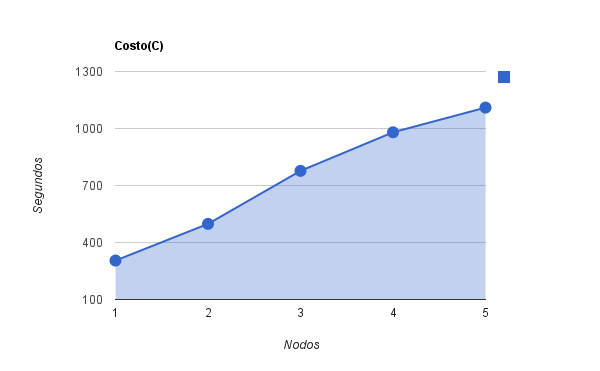
\includegraphics[scale=0.35]{images/Grafico_Costo.png}\\
    \end{minipage}
\end{figure}
\end{center}
\end{frame}

\begin{frame}\frametitle{Otros resultados: tiempos de ejecución}
\begin{center}
\begin{figure}[!ht]

	\begin{minipage}{3cm}
		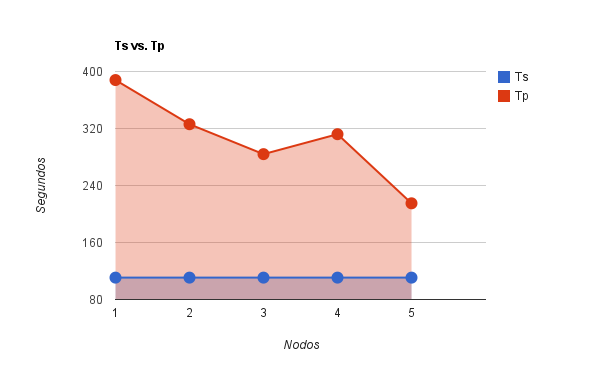
\includegraphics[scale=0.3]{images/grafico_de_tiempos1.png}
    \end{minipage}
    \    \ \hfill
	\begin{minipage}{5cm}
	    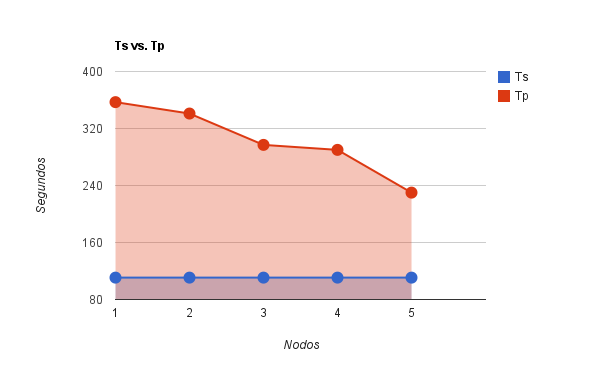
\includegraphics[scale=0.3]{images/grafico_de_tiempos2.png}
	\end{minipage}
\end{figure}
\end{center}

\end{frame}

\end{subsection}


\section{Conclusión y trabajos a futuro}

\begin{subsection}{Conclusión}

	\begin{frame}\frametitle{Conclusión}
		\begin{itemize}\addtolength{\itemsep}{5mm}
			\item La nueva capa de distribución, junto con el rediseño efectuado, mantiene compatibilidad con el modelo original de \fud.
			\pause
			\item Los desarrolladores pueden implementar aplicaciones clientes de FuD-BOINC que pueden correr tanto en 
			Linux como en Windows.
			\pause
			\item FuD-BOINC debería ser utilizado por aplicaciones que requieran gran cantidad de procesamiento.
			\pause
			\item La investigación realizada permitió desenvolvernos satisfactoriamente ante un tema desconocido: computación 
			voluntaria con BOINC.
		\end{itemize}
	\end{frame}

\end{subsection}


\begin{subsection}{Trabajos a futuro}

	\begin{frame}\frametitle{Trabajos a futuro}
		\begin{itemize}\addtolength{\itemsep}{5mm}
			\item Instruir y profundizar los conocimientos sobre la administración y configuración de un proyecto BOINC.
			\item Lanzar oficialmente un proyecto de computación voluntaria \textbf{FuDePAN@HOME}.
			\item Implementar un screensaver con un logo personalizado de FuDePAN.
			\item Agregar la entrega de créditos a los clientes respecto de la cantidad de trabajos procesados.			
		\end{itemize}
	\end{frame}
		
	\begin{frame}\frametitle{Trabajos a futuro}
		\begin{itemize}
			\item Integrar el funcionamiento de las nuevas capas \textbf{L3} y \textbf{L4} de \fud \ con esta capa de distribución.
		\end{itemize}	
		\begin{center}
			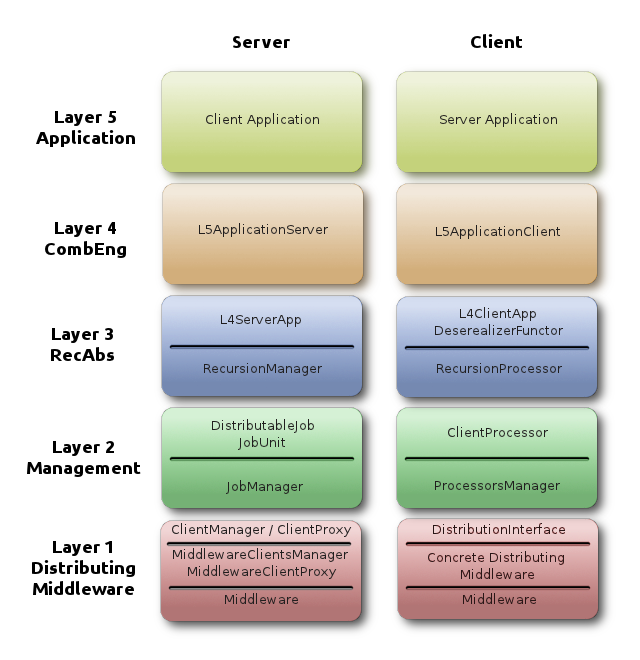
\includegraphics[scale=0.26]{images/fud-l4.png}
		\end{center}
	\end{frame}
	
	\begin{frame}
		\centerline{\Huge{\textbf{¿Preguntas?}}}
	\end{frame}
	
	\begin{frame}
		\centerline{\Huge{\textbf{¡Gracias!}}}
	\end{frame}

\end{subsection}



\end{document}